\documentclass[
  a4paper,
  justified,
  nobib,
  marginals=raggedright,
]{tufte-book}
\usepackage{preambule}

\begin{document}

\frontmatter
\maketitle

% acknowledgements
\cleardoublepage
\thispagestyle{empty}
~\vfill
\vfill
\begin{fullwidth}
\begin{doublespace}
\raggedleft\noindent\fontsize{16}{20}\selectfont\itshape
\nohyphenation
Gorąco dziękuję Magdalenie,\\
bez wsparcia której ta praca nie zostałaby ukończona.
\end{doublespace}
\end{fullwidth}
\vfill

\tableofcontents

\chapter{Przedsłowie}\label{chapter:intro}

\section{Konwencje przyjęte w~niniejszej dysertacji}\label{intro:conventions}

Każdy chemik zauważy, że forma graficzna niniejszej rozprawy doktorskiej różni się
  od~zwykle spotykanych w~naukach chemicznych.
Zapewne najbardziej zwraca uwagę format tekstu \--- 
  jest on~inspirowany pracami Edwarda R.~Tuftego\sidecite{Tufte2001,Tufte1990,Tufte1997,Tufte2006},
  uznanego za~eksperta w~dziedzinie prezentowania informacji i~pioniera wizualizacji
  danych\sidecite{Yaffa2011}.
Tufte zauważa, że odnośniki do~spodu strony, a~tym bardziej końca tekstu,
  utrudniają czytanie, rozpraszając uwagę czytelnika.
Zamiast tego umieszcza przypisy i~komentarze na~szerokim marginesie,
  komentując żartobliwie, że \enquote{to miejsce zaplanował dla nich Bóg}.
Na~takiej szacie graficznej korzysta również główny tekst \---
  zawarty w~kolumnie węższej niż cała strona, ma szerokość uznawaną za~optymalną
  do czytania\sidecite{nanavati05}.

Esencją podejścia Tuftego do prezentowania danych jest położenie nacisku
  na~informatywność, a~nie estetykę przekazu.
Wizualizacja powinna ułatwić jak najlepsze zrozumienie danych w~jak najkrótszym czasie,
  w~jak najmniejszej przestrzeni i~przy użyciu jak najprostszej formy.
Sposób przedstawienia danych musi być jednoznaczny i~nie może ich zniekształcać
  ani wymuszać ich interpretacji.
Dane nie powinny być ozdabiane, a~wszystkie zbędne elementy, takie jak ramki czy tło,
  nie powinny znajdować się na~rysunkach, ponieważ odwracają uwagę od~treści.
Projektując graficzną stronę tego dokumentu starałem się stosować do~tych zasad.

\begin{marginfigure}
  \includesvg{palettes}
  \caption{
    Wykorzystane w~niniejszej dysertacji palety kolorów,
    będące przyjazne osobom z~zaburzeniem rozpoznawania barw.
  }
  \label{fig:palettes}
\end{marginfigure}
Jeden z paradygmatów kształcenia mówi, że nauka, będąc narzędziem poznania,
  powinna być przystępna.
Jako że kolor może nieść istotną część informacji podczas prezentacji danych,
  przy tworzeniu grafik zawartych w~tej pracy użyłem palety przyjaznej osobom
  z~zaburzeniem rozpoznawania barw.
Jako paletę jakościową użyłem schematu kolorów zaproponowanego przez Wonga\sidecite{wong11},
  natomiast jako paletę ilościową wykorzystałem viridis\sidecite{Smith2015} lub BrBG,
  zależnie od~kontekstu.
Wszystkie je prezentuję na~\cref{fig:palettes}.

Na~przystępność tekstu w~ogromnym stopniu wpływa również wybór kroju pisma.
Uważny czytelnik może zwrócić uwagę, że nie jest on jednakowy w~całej objętości
  niniejszej dysertacji.
Wzory chemiczne zapisuję czcionką zalecaną przez organizację \gls{iupac}
  zamiast dominującym, klasycznym krojem szeryfowym.
W~tym miejscu dodam, że doprecyzowując podstawniki ogólne\sidenote{%
    Czyli grupy i~atomy oznaczone jako \ch{X}, \ch{R} lub \ch{R^n}.},
  używam znaku równości (\enquote{$=$}) pokazując konkretne grupy lub atomy,
  a~znaku tożsamości (\enquote{$\equiv$}) prezentując koncepcje\sidenote{%
  Na przykład \enquote{\ch{R}~$\equiv$~alkil} albo \enquote{\ch{R^1}~$\equiv$~\ch{R^2}}.}.

Cyfry występujące w~tekście również nie zawsze wyglądają tak samo.
W~większości są to tak zwane cyfry nautyczne, zaprojektowane tak, aby wizualnie współgrały
  z~minuskułami\sidenote{Czyli małymi litrami.},
  ale do~przedstawienia wielkości fizycznych i~matematycznych użyłem cyfr zwykłych,
  aby zwiększyć ich czytelność.
Podobny zabieg zastosowałem w~przypadku numerów związków występujących w~tekście,
  które są dodatkowo wyróżnione za~pomocą pogrubienia.
Kolejnym odstępstwem jest użycie jaśniejszego koloru do~zapisu cytowań,
  co~pozwala skupić uwagę na~treści, a~nie detalach technicznych.

Pewnie jak większość ludzi parających się naukami ścisłymi ulegam pokusie używania skrótów.
Większość z~nich to~skrótowce standardowo używane przez chemików,
  jednak, dla jasności, wszystkie rozwijam przy ich pierwszym wystąpieniu.
Zgodnie z~konwencją zamieszczam również wykaz tych akronimów,
  wraz z~ich znaczeniem, na~następnych stronach.

Choć główna część tej dysertacji poświęcona jest badaniom z~dziedziny syntezy organicznej,
  podczas pracy nad nią moje zainteresowania poszerzyły się.
Stąd też czytelnik natrafi na~fragmenty dotyczące obliczeń kwantowo\-/chemicznych,
  a~nawet programowania komputerowego.
Zwłaszcza ten ostatni temat wymaga dodatkowego komentarza jako najbardziej oddalony
  od~podstawowej dyscypliny.

Gdy w~tekście pojawia się odniesienie do~nazw elementów opisywanego kodu źródłowego,
  sygnalizuję to~używając kroju czcionki \lstinline!o stałej szerokości!.
Większe bloki kodu są wydzielone z~tekstu, jak ten poniżej.
Dla poprawienia czytelności 
  \lstinline[basicstyle=\ttfamily\color{wongvermillion},columns=fixed]!słowa kluczowe!%
  \footnote{
    Słowa kluczowe to ciągi znaków zarezerwowane w~danym języku programowania,
      stanowiące część jego składni.
    Mają one z~góry określone znaczenie, definiowane przez ten język.
  },
  \lstinline[basicstyle=\ttfamily\color{wongsky},columns=fixed]!komentarze!,
  \lstinline[basicstyle=\ttfamily\color{wonggreen},columns=fixed]!dane tekstowe!, a~także
  \lstinline[basicstyle=\ttfamily\color{wongpurple},columns=fixed]!niektóre zmienne!
  są wyróżnione przy użyciu koloru.
Linie tych bloków są ponumerowane na~lewym marginesie.
Niestety, nie doczekały się one polskiego terminu i~nazywane są \--- 
  z~języka angielskiego \--- listingami.
\Cref{lst:example} jest przykładem takiego bloku kodu.

\begin{listing}
  \begin{lstlisting}
    if is_first_program():
        print('Hello world!')
    else:
        pass  # nic nie rób
  \end{lstlisting}
\caption{Przykład formatowania bloku zawierającego kod źródłowy.}
\label{lst:example}
\end{listing}

Tekst niniejszej rozprawy doktorskiej został przygotowany przy użyciu oprogramowania \LaTeX,
  a~jej kod źródłowy dostępny jest na~dołączonej płycie CD oraz w~Internecie pod adresem \repourl{}.

\section{Cel pracy}\label{intro:goal}
Ramowym celem niniejszej pracy było sprawdzenie, jak współcześnie dostępne metody
  reduktywnej aktywacji amidów sprawdzają się w~roli narzędzi do~syntezy
  sfunkcjonalizowanych amin w~złożonych układach reakcyjnych.
Takie ujęcie zagadnienia, choć obejmuje meritum, zdecydowanie wymaga doprecyzowania.
Wśród badanych przeze mnie \enquote{złożonych układów reakcyjnych} znajdują się dwie,
  wybrane arbitralnie, kategorie.
Pierwszą są reakcje z~amidami posiadającymi grupy estrowe, które w~reakcji reduktywnej aktywacji
  mogą być potencjalnymi konkurentami wobec amidu.
Drugą są reakcje wieloskładnikowe laktamów na~przykładzie pochodnych reakcji Ugiego.
Natomiast do~współczesnych metod reduktywnej aktywacji amidów zaliczam metodę opartą
  o~wykorzystanie bezwodnika triflowego, reakcję z~odczynnikiem Schwartza oraz katalityczne
  redukcje wobec kompleksów irydu \--- kompleksu Vaski i~kompleksu van der Enta.

Za~główny cel postawiłem sobie sprawdzenie, które z~tych metod aktywacji mogą być zastosowane
  do~przekształcenia amidu w~funkcjonalizowaną aminę w~każdym ze~wspomnianych układów
  reakcyjnych oraz jaki jest zakres stosowalności skutecznych procedur.
Podczas jego realizacji natrafiłem na~trudności i~wyzwania, którym starałem się zaradzić,
  wykorzystując metody wykraczające poza standardowo wykorzystywane w~syntezie organicznej.
Dzięki moim zainteresowaniom obejmującym dziedzinę nauk komputerowych,
  mogłem zastosować obliczenia metodami numerycznymi oraz programowanie komputerowe
  do~uzyskania odpowiedzi na~niektóre z~powstałych wątpliwości i~pokonania pewnych przeszkód.
Dociekania te były dla mnie przyczynkiem do~postawienia sobie celów dodatkowych \---
  ustalenia przebiegu wariantu reakcji Ugiego, który badałem oraz stworzenie oprogramowania
  komputerowego, ułatwiającego analizę wyników obliczeń kwantowo-chemicznych.

\section{Publikacje}\label{intro:publications}
\begin{itemize}
  \item \cite{wieclaw21}
  \item \cite{stecko18}
  \item \cite{wieclaw22}
\end{itemize}

\section{Konferencje}\label{intro:conferences}
\begin{fullwidth}
\begin{itemize}
  \item 19\textsuperscript{th}~International Symposium \enquote{Advances in~the Chemistry of~Heteroorganic Compounds}, poster: \enquote{Captodative functionalization of~amidoesters}, Poland, Łódź, 19.10.2016~r.
  \item Ogólnopolskie Studenckie Mikrosympozjum Chemików, wystąpienie ustne: \enquote{Aktywacja amidów na~atak nukleofila jako metoda selektywnej funkcjonalizacji}, Białystok, 30.03.\-–1.04.2017~r.
  \item V~Łódzkie Sympozjum Doktorantów Chemii, poster: \enquote{Aktywacja amidów na~atak nukleofila jako metoda selektywnej funkcjonalizacji}, Polska, Łódź, 11.05.\-–12.05.2017~r.
  \item XIV Warszawskie Seminarium Doktorantów Chemików - ChemSession’17, poster: \enquote{Captodative functionalization of~amidoesters}, Polska , Warszawa, 9.06.2017~r.
  \item 26\textsuperscript{th}~ISHC Congress, poster, Regensburg, poster: \enquote{Chemoselective activation of~amide carbonyls towards nucleophilic reagents}, Niemcy, Ratyzbona, 3.\-–8.09.2017~r.
  \item XX~International Symposium \enquote{Advances in~the Chemistry of~Heteroorganic Compounds} and XVII International Symposiumon on Selected Problems of Chemistry of Acyclic and Cyclic Heteroorganic Compounds, poster: \enquote{Schwartz’s reagent mediated nojirimycin derivatives synthesis}, Polska, Łódź, 23.\-–24.11.2017~r.
  \item XI~Ogólnopolskie Sympozjum Chemii Organiczne, poster: \enquote{Synteza cukrowych pochodnych tetrazoli z~użyciem odczynnika Schwartza}, Polska, Warszawa, 8.\-–11.04.2018~r.
  \item International Congress of~Young Chemists YoungChem~2018, wystąpienie ustne: \enquote{Short and sweet: An~approach to direct synthesis of~iminosugar-derived tetrazoles}, Polska, Bydgoszcz, 10.\-–14.10.2018~r.
  \item XXI~International Symposium \enquote{Advances in~the Chemistry of~Heteroorganic Compounds}, poster: \enquote{An~approach to~direct synthesis of~iminosugar derived tetrazoles}, Polska, Łódź, 23.11.2018~r.
  \item International Symposium on Synthesis and Catalysis~2019, wystąpienie ustne: \enquote{An~approach to~direct synthesis of~iminosugar derived tetrazoles}, Portugalia, Evora, 3.\-–6.09.2019~r.
  \item XXII~International Symposium \enquote{Advances in~the Chemistry of~Heteroorganic Compounds}, poster: \enquote{Iminosugar derived tetrazoles: direct synthesis and mechanistic insights}, Polska, Łódź, 22.11.2019~r.
  \item Virtual Winter Workshop \enquote{Multiscale modeling in materials science, chemistry, and biology: How to meet, greet, and beat scale-bridging challenges}, poster: \enquote{Tesliper: Spectral Simulations Simplified}, Niemcy, Karlsruhe, 22.\--23.11.2021~r.
  
\end{itemize}
\end{fullwidth}

\section{Finansowanie}\label{intro:founding}
\begin{fullwidth}
\begin{itemize}
  \item Grant Preludium \textnumero~2017/25/N/ST5/00079 Narodowego Centrum Nauki
  \item Grant obliczeniowy PL\=/Grid
\end{itemize}
\end{fullwidth}

\begin{fullwidth}
  \printglossary[title=Wykaz skrótów, type=\acronymtype]
\end{fullwidth}
  

\mainmatter
% widths of text elements
% zwykły tekst \printinunitsof{cm}\prntlen{\textwidth}\\  % 10.69847 cm
% margines \printinunitsof{cm}\prntlen{\marginparwidth}\\ %  4.93929 cm
% przerwy \printinunitsof{cm}\prntlen{\marginparsep}      %  0.81987 cm
%                                                 SUMA:     16.45763 cm

\chapter{In litterae}

\section{Trwałość amidów}

\begin{marginfigure}[7\baselineskip]
  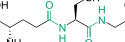
\includegraphics{schemes/glutathione}
  \caption{
    Glutation --- trójpeptyd o~właściwościach przeciwulteniających,
    z~wiązaniami amidowymi zanaczonumi na~zielono.
  }
  \label{fig:glutathione}
\end{marginfigure}
Wiązanie amidowe występuje w~naturze niezwykle powszechnie.
Można nawet pokusić się o~stwierdzenie, że jest ono jednym z~budulców życia ---
w~końcu peptydy, podstawowa struktura biocheniczna złożonych organizmów,
to łańcuchy aminowkasów, połączonych wiązaniami amidowymi.
Za~przykład posłużyć może glutation --- trójpeptyd o~właściwościach przeciwulteniających,
występujący powszechnie w~organizmach roślinnych i~zwierzęcych\autocite{wu04},
przedstawiony na~\cref{fig:glutathione}.
  
\begin{marginfigure}
  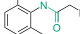
\includegraphics{schemes/lidocaine}
  \caption{
    Lidokaina --- przykład leku posiadającego ugrupowanie amidowe
    (zaznaczone na~zielono).
  }
  \label{fig:lidocaine}
\end{marginfigure}
Ugrupowanie to~można też znaleźć w~wielu związkach biologicznie czynnych.
Za~prosty przykład niech posłuży lidokaina, przedstawiona na~\cref{fig:lidocaine},
powszechnie stosowana jako środek miejscowo znieczulający.
Przykładów takich możnaby przytoczyć wiele, bo~jak pokazuje analiza produkcji farmaceutyków,
\SI{66}{\percent} leków syntezuje się tworząc wiązanie amidowe\autocite{carey06}.

W~latach 30. ubiegłego wieku firma DuPont wprowadziła na~rynek poliamidy na~rynek tworzyw sztucznych pod nazwą handlową Nylon.
Ten bardzo trwały materiał szybko znalazł zastosowanie w~wielu gałęziach przemysłu.
Stosuje się go przede wszystkim do~wytwarzania syntetycznych włókien tekstylnych,
ale też do~produkcji szczoteczek do~zębów, strun do~instrumentów, żyłek wędkarskich, czy opakowań żywności.


Tę powszechność --- zarówno wśród produktów naturalnych, jak i~wytworów cywilizacji ---
amidy zawdzięczają między innymi swojej wyjątkowo niskiej reaktywności.
Wiązanie amidowe ulega niewielu przemianom chemicznym, a~jeśli już, to~
zwykle wymaga stosowania bardzo ostrych warunków prowadzenia reakcji.
Ta niezwykła trwałosć wynika z~bardzo efentywnego nakładania się orbitali 
molekularnych atomu azotu oraz $\pi$ wiązania podwójnego \ch{C=O}.
Pozwala to na~wydajną delokalizację elektronów w~obrębie wiązania i~znaczny 
udział dwóch możliwych struktur dipolarnych, jak widać na~\cref{sch:resonance}.
\begin{scheme}
  \centering
  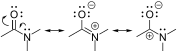
\includegraphics{schemes/resonance}
  \caption{
    Struktury rezonansowe wiązania amidowego, zapewniające mu~niezwykłą trwałość.
  }
  \label{sch:resonance}
\end{scheme}


\section{Prezkształcenia amidów}
Już w~drugiej połowie XIX~w. chemicy wiedzieli, że pierwszorzędowe amidy mogą ulegać reakcji odwodnienia, dając nitryle.
Z~roku \citeyear{wallach77} pochodzi publikacja dotycząca odwadniania amidów drugorzędowych.\autocite{wallach77}
Jej autorom udalo się tego dokonać dzięki zastosowaniu \ch{PCl5} jako reagenta.
To doniesienie jest pierwszą publikacją na temat przekształceń amidów, jakią można znaleźć w dostępnej literaturze.

\begin{marginscheme}
  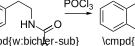
\includegraphics{schemes/bichler}
  \caption{Ogólny schemat reakcji Bichlera-Napieralskiego.}
  \label{sch:resonance}
\end{marginscheme}
W~\citeyear{bischler93} \citeauthor{bischler93} pokazali, że działając \ch{POCl3}
na~amid wywiedziony z~\iupac{2-fenyloetyloaminy} można otrzymać pochodną dihydroizochinoliny\autocite{bischler93}.
Jakiś czas później wariację tej przemiany pokazali \citeauthor{pictet10}.
Wychodząc z~\iupac{2-hydroksy-2-fenetyloamidu} otrzymali w jednym etapie produkt już odwodniony - izochinolinę.\autocite{pictet10}
W~roku \citeyear{vilsmeier27} \citeauthor{vilsmeier27} pokazali, że reakcję tę można prowadzić nie tylko wewnątrzcząsteczkowo,
nie da się jednak zatrzymać jej na etapie addycji do~arenu.
Realcja \iupac{N,N-dimetyloamidu} z~\ch{POCl3} prowadzi do~powstania kationu chloroiminiowego, nazywanego też reagentem Vilsmeiera.
Ulega on addycji do bogatych w elektrony arenów, tworząc iminę.
Podczas przerobu reakcji następuje hydroliza tego adduktu, skutkując powstaniem odpowiedniego aldehydu (lub ketonu) arylowego\autocite{vilsmeier27}.
\begin{scheme}
  \centering
  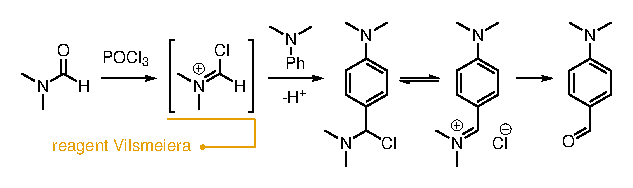
\includegraphics{schemes/vilsmeier}
  \caption{Mechanizm reakcji Vismeiera-Haacka.}
  \label{sch:vilsmeier}
  \setfloatalignment{b}
\end{scheme}


Przez długi czas chemia amidów była raczej uboga ---
ograniczała się przede wszystkim do~prostych reakcji, dziś uznanych za~podręcznikowe.
W~pierwszej kolejności można wymienić ich redukcję do~amin oraz hydrolizę.

\section{Odczynnik Schwartza}


\chapter{In vitro}

\chapter{In silico}
\section{Obliczenia mechanizmu}
\section{Symulacja widm}

\chapter{In machina}
\section{Istota programu}
\section{Wybór języka programowania}

\chapter{In detail}
\section{Procedury}
\section{Analizy}

\backmatter

% \printbibliography

\end{document}
